%!TEX root = ../thesis.tex
%*******************************************************************************
%****************************** Literature review chapter *********************************
%*******************************************************************************


\chapter{Background Knowledge and Related Work}\label{chapter:Background}
%What I really want to outline here is that I am reviewing work related to a pretty narrow field - that of target detection in a forensic management scene. After giving some broader information related to multi-agent systems etc., give a narrower summary of work in this field.

\workinprogress
As mentioned in the introduction chapter, the research outlined in this thesis was motivated and funded by an EU Horizon 2020 project called ROCSAFE, which involves investigating the automation of certain aspects of the management and examination of a crime scene in the forensic stage of analysis. Accordingly, this chapter outlines existing research specifically related to the application of agent-based systems in this area, while also providing a broad overview of single and multi-agent systems and general techniques commonly used in such systems to solve abstract problems. \par
First, a synopsis of the ROCSAFE project, which funded and motivated this work is presented. Then a broad overview of agent-based systems is given, mainly outlining common approaches in agent and multi-agent system design. This leads to a more focused discussion on how agents and multi-agent systems have been designed in work that is tightly related to that of this thesis. Important concepts and algorithms relating to multi-agent probabilistic search and multi-agent coverage are then outlined. Techniques used to reach the current state-of-the-art for these problems are identified and discussed. Finally, work previously done 
%in simulating environments for systems that operate in a complex real-world scenario is appraised and reviewed.
which relates to the research questions stated in Chapter \ref{chapter:introduction} is appraised and reviewed.

\section{The ROCSAFE Project}\label{sec:ROCSAFEBG}
\note{not sure how deal with double acronym in ROCSAFE}
\textbf{R}emotely \textbf{O}perated \textit{\textbf{C}hemical, Biological, Radiation, Nuclear, explosive (CBRNe)} \textbf{S}cene \textbf{A}ssessment and \textbf{F}orensic \textbf{E}xamination (ROCSAFE) is an EU Horizon 2020 project. Horizon 2020 is an EU Research and Innovation Program, with almost €80 billion in total funding allocated from 2014 to 2020. The ROCSAFE project comes under the \textit{Secure societies - Protecting freedom and security of Europe and its citizens} programme, whose objective is \textit{"to foster secure European societies in a context of unprecedented transformations and growing global interdependencies and threats, while strengthening the European culture of freedom and justice".}
\href{https://cordis.europa.eu/programme/rcn/664463/en}{ }\footnote{\href {https://cordis.europa.eu/programme/rcn/664463/en}{https://cordis.europa.eu/programme/rcn/664463/en}}

Specific details of the ROCSAFE project can be found at the \href{https://cordis.europa.eu/project/rcn/203295/factsheet/en}{Horizon 2020 website}\footnote{\href {https://cordis.europa.eu/project/rcn/203295/factsheet/en}{https://cordis.europa.eu/project/rcn/203295/factsheet/en}} 
and 
\href{http://rocsafe.eu/}{ROCSAFE website.}\footnote{\href {http://rocsafe.eu/}{http://rocsafe.eu/}}. We summarise the relevant details here, based on these primary sources. The high-level goal of ROCSAFE is to fundamentally change how CBRNe events are assessed, given that current practices require personnel to enter hazardous areas with unquantified risks. The project does not aim to provide a first response to CBRNe events; rather it intends to provide support to the forensic phase of the investigation, which is chiefly concerned with the collection, preservation, and scientific analysis of evidence during the course of an investigation, ideally leading to the ability to present admissible evidence during a criminal investigation. 
%It is worth noting that forensic investigations are not particularly time-sensitive; for large-scales scenarios they can typically last for months or years.\note{would be good to find a source for this}\par


CBRNe events are exceedingly difficult to prepare for because they are so rare and diverse, with the consequence that limited data from real events is available to use as a reference. Despite this, many of the procedures related to forensic investigations are well-defined, in order to preserve the chain-of-custody of evidence. The work done in this thesis was identified at the inception of the project to aid: 
\begin{enumerate}
    \item The initial phase of the forensic investigation, in which a survey of the scene is carried out in order to provide high-level information related to the examination area to the crime scene manager.
    \item The identification and localisation of forensic evidence that can be detected using sensors developed as part of the project.
    \item Prototyping, testing and validation of some of the technologies related to this project. This was done by designing a high-fidelity simulation environment from scratch.
\end{enumerate}





\section{Agents and Multi-Agent Systems}
This section provides some general background knowledge related to intelligent agents and multi-agent systems. We introduce common terminology and outline approaches that are commonly taken when designing agents.
%talk about the usual design of multi-agent systems and the history of multi-agent systems
%introduce some nomenclature
\nomenclature[Y]{Percept}{A percept is an interpreted reading of the state of the environment, taken by the agent's sensor}
\nomenclature[Y]{Action}{An action is ...}
\nomenclature[Y]{State}{A state is ...}
\nomenclature[Y]{Utility function}{A utility function is a function that maps a sequence of states to a real number. It is used to give a value to the outcome of actions. }
\nomenclature[Y]{Performance Measure}{A performance measure is }
\nomenclature[Y]{MAS}{Multi-Agent System}

\subsection{Agency} \label{AgencySubsection}
An essential concept which is repeatedly referred to in this thesis is that of an \emph{agent}. The term "\textit{agent}" is an abstract one with no single definition universally accepted in the literature. Most definitions agree reasonably closely with the one provided in AI: A Modern Approach by Russell and Norvig: an agent is "\textit{anything that can be viewed as perceiving its environment through sensors and acting upon that environment through actuators.}"\cite{AIAMA}.  Figure\ref{fig:agent_env_interaction} helps to illustrate this concept. 
\begin{figure}
    \centering
    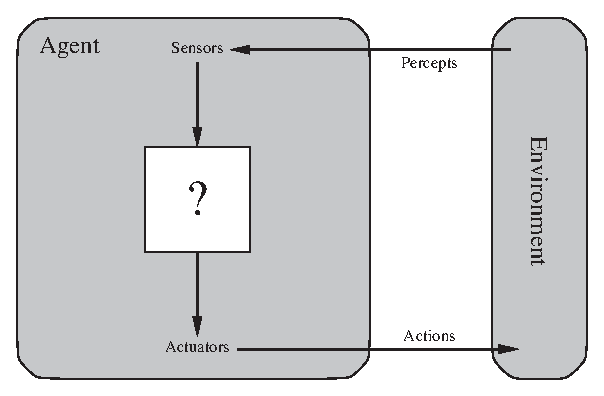
\includegraphics{Chapters/BackgroundKnowledgeAndRelatedWork/Figs/Vector/agent-environment.eps}
    \caption{Agent-Environment Interaction (Russell and Norvig)\cite[p.~35]{AIAMA}}
    \label{fig:agent_env_interaction}
\end{figure}
The box containing the question mark represents the agent's internal decision-making process, which generally speaking involves choosing an action, given the complete history of everything that the agent has perceived. The mapping from percept sequences to actions is described as the agent function. The agent function is an abstract notion; at a lower level an agent program implements the agent function, running on some physical system. A key concept in developing an agent program is rationality: "\textit{for each possible percept sequence, a rational agent should select an action that is expected to maximize its performance measure, given the evidence provided by the percept sequence and whatever built-in knowledge the agent has}"\cite[p.~37]{AIAMA}. This thesis is concerned with designing a system of agents that should exhibit rational behaviour.\newline
 

Russell and Norvig group agents into four common classes based on the design of the agent function\cite[p.~47]{AIAMA}: 
\begin{enumerate}
    \item \textbf{Simple reflex agents}: These agents select actions to take by ignoring the percept history to date, with the exception of the most recent percept.
    \item \textbf{Model-based reflex agents}: These agents have an internal state that depends on the percept history and is updated using new percepts. Updates occur using a model of the world.
    \item \textbf{Goal-based agents}: These agents are an extension to model-based reflex agents. They have some information about whether they have reached a "goal" state, which is desirable. The agent can choose actions to take based on the model. \note{Define what a goal state is.}
    \item \textbf{Utility-based agents}: A utility function is used as an internal performance measure in order to select actions. This allows an agent to pick among actions that may not immediately lead to a goal state.
\end{enumerate}
Recent work in the field of AI has strongly focused on learning agent architectures, which is a superset of all of the above agents. The key difference between the agent types listed above and a learning agent is that a learning agent has the ability to improve its performance through time independently. Its decision making process is not necessarily static and can change beyond its initial programming. An explanation of the architecture of a learning agent can be found in Russell and Norvig \cite[p.~55]{AIAMA}. Implementing each of these different types of agents requires varying degrees of effort. Depending on the problem, different architectures may be more or less suited, which suggests that fully understanding the problem that is attempted to be solved is of fundamental importance when designing an agent.

\subsection{Multi-Agent Systems}
Analogous to the definition of an agent, there is no universally agreed-upon definition of a \emph{Multi-Agent System} (MAS). A definition is provided in a field review paper by Stone and Veloso: "\textit{Multiagent Systems (MAS) is the subfield of AI that aims to provide both principles for construction of  complex  systems  involving  multiple  agents  and  mechanisms  for  coordination  of  independent  agents’ behaviors}" \cite{Stone2000MultiagentPerspective}. While the design of individual agents tends to focus on maximising a performance measure, the design of a multi-agent system is rather more multi-faceted. Weiss \cite{MAS:AModernApproachToDAI} notes that it is almost always oriented towards answering the question of "\textit{when and how to interact with whom}". Multi-agent systems have been proposed as a solution to many problems that modern AI attempts to tackle for some of the following reasons, which are outlined in more depth in \cite{Stone2000MultiagentPerspective}: 
\begin{itemize}
    \item Some problems by definition can be described as a multi-agent system. An example is an organization that may want to model it's internal affairs with a single system. The different departments have their own sub-systems that have differing priorities and capabilities; their interactions naturally can be thought of as interactions between independent agents, in accordance with the definition provided at the start of this section.
    \item The accomplishment of a task can be expedited significantly by using multiple agents. Multi-agents systems are part of the field of Distributed Artificial Intelligence (DAI) and so problem domains that decompose into several independent tasks that can be handled by separate agents can benefit from their use. The problem of efficient task allocation in multi-agent systems has been well-studied in the literature\cite{Gerkey2004ASystems}. 
    \item Robustness is an often-cited benefit of multi-agent systems. Distributed control means that failure of a single agent (mechanical or otherwise) may be tolerated.
    \item Multi-agent systems are often more scalable than single-agent systems. The necessary modularity of multi-agent systems means that adding new agents to the system can often be a solution to a more difficult problem, rather than adding new capabilities to a monolithic system. 
    \item The modularity of multi-agent systems means that the design and programming of them may be simplified. For example, rather than solving a multi-objective problem with a single agent, a single-objective problem may be solved with multiple agents. A result of this is that multiple cheap robots may be used to outperform a single, expensive robot \cite{Grabowski2000HeterogeneousExploration}.
\end{itemize}
\par



\section{High Fidelity Simulation Environments}
In this section, we discuss existing literature and common approaches related to designing and implementing high-fidelity simulation environments. This provides a backdrop for Chapter \ref{chap:HighFidelitySim}, which describes the work we did to implement our own custom high-fidelity simulation environment.
\subsection{High Fidelity Simulation Environments Related Literature}\label{sec:SimulationEnvironmentsRelatedLiterature}
%Want to introduce the problem to allow for a discussion that makes sense. Ideally will frame a problem so that it suggests that having a high-fidelity simulation environment would be very useful for the project and in general.
%\nomenclature[]{UUV}{Unmanned Underwater Vehicle}
\subsection{Key Aspects of Simulation Environments}
We begin by discussing some key aspects of simulation environments that serve as a starting point on which more advanced techniques build upon. According to %\citeauthor{Shannon1998INTRODUCTIONSIMULATION} 
\citeauthor{Shannon1998INTRODUCTIONSIMULATION}, simulation can be defined as \textit{"the process of designing a model of a real system and conducting experiments with this model for the purpose of understanding the behavior of the system and/or evaluating various strategies for the operation of the system"} \cite{Shannon1998INTRODUCTIONSIMULATION}. Simulations have been used extensively to model complex systems since the invention of the modern computer, gaining traction since the proposal of the Markov Chain Monte Carlo method by Stansislaw Ulam and John Von Neumann in the late 1940s \cite{Robert2011AIncomplete}. Simulations written with software are created in order to gain insight into the system's dynamics and to evaluate results of using a method intended for real-world use. This is usually because proposed methods may be too time-consuming or expensive to test in the real world. Software simulations are being used increasingly for a wide variety of tasks, from planning new roads to alleviate traffic \cite{Pell2017TrendsSimulation} to developing self-driving vehicles \cite{Dosovitskiy2017CARLA:Simulator}. 

Designing simulations allows the developer of an agent-based system to abstract away details of the real-world conditions that the agents will act in and focus on the salient aspects that the agents are concerned with, in order to prototype, train, test, analyse and validate. General advantages of simulations are listed in  \cite{Shannon1998INTRODUCTIONSIMULATION}, with the most notable being:
\begin{itemize}
    \item \textit{"It can be used to explore operating procedures, decision rules, organizational structures, etc. without disrupting the ongoing operations."}
    \item \textit{"Simulation allows us to control time. Thus we can operate the system for several months or years of experience in a matter of seconds allowing us to quickly look at long time horizons or we can slow down phenomena for study."}
    \item \textit{"It allows us to gain insights into how a modelled system actually works and understanding of which variables are most important to performance."}
    \item \textit{"Simulation's great strength is its ability to let us experiment with new and unfamiliar situations and to answer "what if" questions."}
\end{itemize}


\note{Following paragraph doesn't really belong here but does help tie everything together}

 In relation to designing intelligent agents, often the trade-off between exploration and exploitation is referenced. Exploration or "information gathering" \cite{AIAMA} can be considered as the agent posing a "what if" question in order to learn the consequences of performing action, and exploitation can be considered as an agent using gathered or previous knowledge to choose actions to take that maximize its performance measure, as outlined in Section \ref{AgencySubsection}. Since simulation environments are highly suited to answering "what if" questions, which has motivated the use of using simulations to design systems of autonomous agents in the literature, for example the simulation environment used in the 
\href{https://multiagentcontest.org/}{Multi-Agent Programming Contest.}\footnote{\href {https://multiagentcontest.org/}{https://multiagentcontest.org/}}



\subsection{Simulation Environments Design Using Game Engines}\label{subsec:GameEngineReview}
Since computer games are effectively simulations, the technologies used to create them have also been used to create simulations for a more serious purpose, often referred to in the literature as \textit{serious games}. Serious games usually refer to games that have been specifically designed to provide training to professionals working in an industry where extensive training is necessary but difficult, expensive or dangerous to provide \cite{Sobke2016SeriousEngines}. An overview and taxonomy of serious games is provided by \citeauthor{Laamarti2014AnGames} \cite{Laamarti2014AnGames}. Early motivation for using games engine in scientific research is outlined in a 2002 journal article by \citeauthor{Lewis2002GameEnginesInScientificResearch}, summarized by the sentence "\textit{By elevating the problems of updating and synchronization to a primary concern, game engines provide superior platforms for rendering multiple views and coordinating real and simulated scenes as well as supporting multiuser interaction}" \cite{Lewis2002GameEnginesInScientificResearch}.  More recently, games have been used to train learning agents, defined in Section \ref{AgencySubsection}. The reasons that this is a recent phenomenon are as follows:
\begin{itemize}
    \item
    As discussed in Section \ref{AgencySubsection}, training a learning agent usually involves defining a mapping from environment states or percept sequences to actions, in order to maximize the performance measure. Until a few years ago, state-space representations of many environments were of such a high dimension that it was prohibitive to find such a mapping. Seminal works on Neural Networks \cite{Lecun1998Gradient-BasedRecognition}, \cite{Krizhevsky2012ImageNetNetworks} have allowed high-dimensional states to be compressed to lower-dimensional ones while retaining key information related to the states, simplifying the process of mapping states to actions. This has led to the development of algorithms that can utilise high-dimensional states to choose optimal actions to great effect, such as Deep Q-Learning \cite{Mnih2013PlayingLearning}.
    \item Writing complex software simulations rendering high-fidelity sensor outputs (e.g. images) in order to train an agent requires a lot of highly-optimised code, which takes a significant amount of effort to write.
    %Issues such as synchronization are non-trivial to resolve. 
    General Purpose Graphics Processing Units (GPGPUs) have significantly decreased the time required to carry out certain tasks in parallel, which has made the problem of calculating sensor outputs in a reasonable time tractable. For example, the rendering time for photo-realistic images has significantly sped up relative to the rendering time using a CPU only \cite{Ryoo2008OptimizationCUDA}.
    \item Insufficient amounts of data could be generated in a reasonable amount of time for the learning agent to perform sufficiently well. Quicker CPU speeds have increased the rates at which agents can learn significantly over the last number of years, in agreement with the predictions of Moore's law \cite{MacK2011FiftyLaw}. Game engines tend to have highly optimised code and given the possibility to generate copious amounts of data in a small amount of time, they have significantly expedited the rate at which learning agents can be trained \cite{Juliani2018Unity:Agents}, \cite{Sadeghi2016CADImage}. 
\end{itemize}
%\note{Should really have citations for all of the above.}

There have been some highly notable simulation environments written with various games engines for non-gaming purposes. One of the first mature simulations written for a serious purpose using technologies usually applied to game development is the Gazebo simulator \cite{Koenig2005DesignSimulator}. Gazebo makes use of physics engines and graphics rendering engines that are commonly used to develop games. The use of Gazebo has been reported to reduce the training time for some simple benchmark robotics tasks by as much as 33\%, while retaining the same level of performance \cite{Vilches2018RobotGazebo}. 

There have also been a notable number of simulators designed to aid the development of autonomous cars, trucks, RAVs and UUVs, with documentation on each commonly citing difficulties in changing configurations for physical vehicles, time taken to generate data and dangerous edge cases as motivation \cite{Dosovitskiy2017CARLA:Simulator}, \cite{Wymann2015TORCS:Simulator}, \cite{Shah2017AirSim:Vehicles}, \cite{Bojarski2016EndCars}. \citeauthor{Dosovitskiy2017CARLA:Simulator} designed the CARLA open-source simulator \cite{Dosovitskiy2017CARLA:Simulator} for autonomous driving research using Unreal Engine 4 (UE4) to provide a lot of basic functionality. They cite "\textit{state-of-the-art rendering quality, realistic physics, basic NPC logic, and an ecosystem of interoperable plugins}" as key motivations to use the engine. AirSim \cite{Shah2017AirSim:Vehicles} is also built over UE4, with their motivations including
\begin{itemize}
    \item "\textit{The amount of training data needed to learn useful behaviors is often prohibitively high}".
    \item "\textit{Autonomous vehicles are often unsafe and expensive to operate during the training phase}".
    \item "\textit{Simulated perception, environments and actuators are often simplistic and lack the richness or diversity of the real world}".
    \item It is "\textit{important to develop more accurate models of system dynamics so that simulated behavior closely mimics the real-world}".
\end{itemize}
\note{maybe just keep comma-separated list}

Finally, the designers of Sim4CV \cite{Mueller2016ATracking}, which is also built over UE4, list the following motivations for the work done in developing a simulation environment for RAV tracking:
\begin{itemize}
    \item "\textit{The combination of the simulator with an extensive aerial benchmark provides a more comprehensive evaluation toolbox for modern state-of-the-art trackers and opens new avenues for experimentation and analysis.}"
    \item \note{not sure how to deal with quoted citations} "\textit{Although simulation is popularly used in machine learning and animation and motion planning, the use of synthetically generated video or simulation for tracker evaluation is a new field to explore.}"
    \item "\textit{The Unreal Engine 4 (UE4) has recently become fully open-source and it seems very promising for simulated visual tracking due in part to its high-quality rendering engine and realistic physics library.}"
    \item "\textit{Our proposed RAV simulator along with novel evaluation methods enables tracker testing in real-world scenarios with live feedback before deployment}"
\end{itemize}
\note{Some of the above can be removed, only need most important points.}

\subsection{Software Simulations Related to Hazardous Scenes}\label{subsec:RelatedSimulations}
\note{Talk about USARSim and others}
%hazardous scenarios are the main focus of ROCSAFE. They are diverse. Simulating them is of high value as already outlined - principally due to dangerous element. Talk about previous work that simulates hazardous scenes and how 
We now move the discussion to the domain of hazardous scenario management. There are a number of existing software simulations that were designed to aid the management of hazardous scenarios. In this context, the scenarios are taken to be of a very serious nature, such that there is an immediate and unquantified risk to human life in the immediate vicinity.

\par \citeauthor{Jacoff2003TestRobots} provide a review of the design process of physical search and rescue environments in an urban setting with the aim of aiding the design of robotic navigation systems \cite{Jacoff2003TestRobots}. They discuss the recommended physical configuration of simulation environments and offer technical details on how the simulation could be run, including performance metrics and details of how the robot should interact with the environment. The details are relatively high-level, but serve as a good starting point on which to develop more complex and realistic scenarios.

USARSim \cite{Carpin2007USARSim:Education} was proposed in 2007 as a general-purpose simulation environment for Urban Search-and-Rescue (USAR) scenarios. It was built using Unreal Engine 2 and was designed to specifically facilitate the design and testing phase of autonomous robots that would be used to help deal with dangerous scenarios. The simulator was designed to be used as a companion to the National Institute of Standards’ (NIST) Reference Test Facility for Autonomous Mobile Robots for Urban Search and Rescue. They describe the decision to use a game engine as their simulation platform as one that considers the strong advantages of offloading the most technical and difficult aspects of simulation to the game engine, which provides superior visual rendering and physical modelling. This allows the user to concentrate their efforts on developing the robotics-specific tasks related to the management of the scenario.\par


VIVID: Virtual Environment for Visual Deep Learning \cite{Lai2018ViviD:Learning} is a set of integrated tools that is capable of generating photo-realistic quality images and sensor readings from simulated vehicles. It was designed using UE4 and ships with a number of ready-made environments. The author envisages its main applications as lying in the domains of "\textit{deep reinforcement learning, semantic segmentation, object recognition, action recognition and video event detection.}" A number of the ready-made environments involve a hazardous component which could benefit from autonomous scene surveying and management, such as the ruined school and train station scenarios.


%This is because game engines have reached a level of maturity that can provide high-fidelity percepts to agents in order to replicate the true environment they would like to perform in. 

%I don't think this is relevant enough to include
%Initially, industries such as manufacturing created a demand for simulation technology, since taking a manufacturing plant offline in order to integrate new robotics technology could cost a company a significant amount of money. Simulink, developed by Matlab, was a popular tool to develop models of dynamical systems, but it's limitations include ...


%Modern-day games are commonly written using a \textit{game engine}, rather than being designed from the bottom up as a singular entity. There is no strict definition for what constitutes a game engine, but the term usually describes a software development environment which typically provides functionality including some kind of rendering engine for 3D graphics, a physics engine that deals with phenomena such as collision, a sound engine, networking abilities, memory management, threading, cinematics and animation. This functionality is necessary in most modern games and has been developed to economise the process of game development.\par



%\subsection{AirSim Simulator}

%We have identified the following aspects of the real-world scenario we hope to address as causing issues in developing our system:
%This motivates the development of a high-fidelity simulation to circumvent these limitations.



%Simulations are typically of high value when data required to design system:
%\begin{itemize}
%    \item Costs a lot of money to generate.
%    \item Is dangerous to generate.
%    \item Is time consuming/laborious to generate.
%    \item The system has a well-known stochastic element which makes generating a sufficiently large sample size difficult.
%\end{itemize}
%The domain which motivated the development of the technologies proposed in this thesis satisfies all of the above requirements, which naturally motivates the design of a simulation environment. \par

% Key properties of a simulation 

%Intelligent agents are frequently designed to solve problems which usually would be on or more of: labour intensive, monotonous, repetitive or time consuming. In order to accomplish these tasks, agents may need to use data from 

%Simulation environments are used to solve a number of different problems when using intelligent agents.

%A consequence of this is that any systems that are developed to provide support can be difficult to evaluate and validate. To address this, we developed a high-fidelity simulated environment as part of the research involved in this thesis, which preserves the critical aspects of CBRNe incidents without presenting any risk of exposure to the dangerous elements of such scenes in the real world. The following published works related to the development of the simulation environment are discussed in this chapter: \citet{Smyth2018AInvestigation}, \citet{Smyth2018UsingDrones}.\par


%Virtual environments designed using games engines have previously been used to gather data to train models for a range of applications \cite{1608.02192}\cite{uav_benchmark_simulator} and software packages have been written that can generate photo realistic images from games engines\cite{1609.01326}. There have also been attempts made to develop models of physical systems that simulate potentially dangerous environments \cite{4625089}. To the best of our knowledge, there are no prior applications using games engines to model critical incidents for the purpose of developing analytical tools in a virtual setting that will then transfer to real-world deployment.

\section{Stochastic Target Localisation Related Literature}\label{sec:StochasticTargetLocalisationRelatedLiterature}



This section discusses the literature related to the problem of target localisation, pertaining to the first research question in Section \ref{sec:ResearchQuestions}. The necessary background knowledge to fully understand these approaches is provided in the next section (Section \ref{sec:StochasticTargetLocalizationBackground}).\par


We state problem of stochastic target localisation in a general setting as follows:
\\
\\
   \textit{ Given a region of space to explore and a set of heterogeneous autonomous aerial vehicles with sensing capabilities, devise a search strategy with a search cutoff criteria which will accurately return either the locations of the targets if one or more is present, or return that no targets are present, in the shortest possible time.}
\\
\\
\par The problem and its variants have been studied extensively and we survey the existing literature behind it here in chronological order. The study of problem can be traced back to a series of three papers by \citeauthor{KoopmanTheoryOfSearchTargetDetection} \cite{Koopman1956THEBASES}, \cite{KoopmanTheoryOfSearchTargetDetection}, \cite{Koopman1957TheEffort}. The first of the three, entitled "Kinematic Bases", references World War $\Romannum{2}$ as a primary motivation behind the series, citing "\textit{detection, location, and identification of targets}" as a key problem which required an urgent solution \cite{Koopman1956THEBASES}. Three key general features of search are identified, which are addressed individually in each of the three papers:
\begin{enumerate}
    \item "\textit{Kinematic Bases}" addresses search with a focus on the kinematic constraints involving the positions, geometric configurations and motion of the seachers and targets \cite{Koopman1956THEBASES}.

    \item "\textit{Target Detection}" is concerned with the stochastic nature of the sensors and instrumentation that is used when navigating and detecting \cite{KoopmanTheoryOfSearchTargetDetection}.
 
    \item "\textit{The Optimum Distribution of Searching Effort}" examines the probability of contact under the stated conditions. It also provides insight on how to optimise results by choosing a search strategy which maximises the probability of contact \cite{Koopman1957TheEffort}.
\end{enumerate}
\par This introduced the problem in structured manner and offered a strong insight into potential future research. In subsequent years the research branched into problems that involved the motion of both the searchers and the target \cite{Stone1980OptimalTargets}, or just the searchers \cite{Chew1966AProcedure}. Since the work in this thesis is primarily concerned with stationary targets, we refer the reader to the PhD. thesis \cite{Lau2007OptimalEnvironments} for a broad review of the literature related to search with a moving target. 

\citeauthor{Chew1966AProcedure} explored an instance of the search problem which is very close to the version this thesis explores \cite{Chew1966AProcedure}. The following assumptions were made
\begin{itemize}
    \item There is an object to be found in one of $R$ boxes at discrete locations or an $R+1^{st}$ representing the absence of the object.
    \item Sampling locations for the objects returns values with a false negative rate $\alpha_i$, which depends on the location.
    \item The boxes at discrete locations can be searched sequentially.
    \item All outcomes are independent, conditional on the location of the object and the search procedure used.
    \item A loss function introduces a cost for concluding the search when the object has not been found.
\end{itemize}
Note that no false positives were assumed to be observed. A dynamic programming approach was proposed, based on \cite{Blackwell1961DiscreteProgramming}, which was shown to be optimal when restricted to a fixed number of inspections. In this case, "optimal" is taken to mean that the strategy minimises the searcher's total expected cost of searching and stopping. A stopping rule was also suggested, with a proof of desirable properties such as minimizing expected cost when using an optimal search procedure.

\citeauthor{Black1965DiscretePROBLEM} examined a discrete instance of the stochastic target localisation problem for a stationary target, following the similar assumptions as \cite{Chew1966AProcedure} above, with the exception of the possibility of the object not being present (represented by the $R+1^{st}$ location) and without a cost for concluding the search when the object has not been found \cite{Black1965DiscretePROBLEM}. A sampling policy was proposed that was shown to be optimal in terms of minimising the expected cost of the search, according to an arbitrary cost function. The optimal policy was summarised as "\textit{Always look in the region for which the posterior probability (given the failure of earlier looks) of finding the object divided by the cost is maximum.}". The policy was not described in terms of a dynamic program, which the author claims provides more transparency to the solution, as opposed to previous work.

\citeauthor{Ross1969AStop} examined the search problem with the assumptions set out in \cite{Chew1966AProcedure} with the exception of the possibility of the object not being present (represented by the $R+1^{st}$ location) but did include the issue of when to conclude the search \cite{Ross1969AStop}. The paper showed that in general, an optimal search strategy exists for the problem with a penalty cost for stopping the search. He proved that when searching is warranted (i.e. the cost of stopping is small relative to the cost of further searching), the optimal search strategy is the same as in the no-penalty case. This means that to optimally solve the general problem of searching and stopping when a penalty cost for stopping is charged (as set out in \cite{Chew1966AProcedure}), the only additional requirement to the use of the optimal search strategy is a stopping time s* that is optimal when used with that search strategy.

\citeauthor{Chew1973OptimalProblem} then iterated on his previous work \cite{Chew1966AProcedure} and outlined a best stopping rule to accompany the optimal search procedure described in \cite{Chew1966AProcedure} with the work in \cite{Chew1973OptimalProblem}. This went a step further than \cite{Ross1969AStop}, since it included the possibility that the object is not present in the search region. The optimal stopping rule was found to be derived from the optimal dynamic programming strategy outlined in \cite{Chew1966AProcedure}, subject to a realistic technical condition relating the search termination cost, the cost of searching each location and the probability of a missed detection in each location.

\citeauthor{Kimeldorf1979BinomialObjects} studied the more general problem of locating $n$ objects hidden among $m$ boxes, where $m$ is known and $n$ is unknown \cite{Kimeldorf1979BinomialObjects}. They assume that there is a cost associated with searching each box and that the distributions of $p$ (the number of boxes) and $\pi$ (the distribution objects among the boxes) are known. They also assume that they know when all the objects have been found and that there is no associated search termination cost. Their results showed that for special cases of the distributions of $n$ and $p$, optimal search strategies can be found which are an extension of the general strategy set out in \cite{Blackwell1961DiscreteProgramming}.\par \citeauthor{Assaf1985OptimalApproach} tackled the same problem, but imposed the constraint that the distribution of $\pi$ is not known exactly, but instead some partial information is known about $\pi$ \cite{Assaf1985OptimalApproach}. Their findings showed that even small random fluctuations, or statistical inaccuracies, may give rise to results that are greatly different from the results obtained when $\pi$ is perfectly known. This suggested that a robust strategy in the case of a possibly inaccurate knowledge of $\pi$ would be desirable.

Many recent approaches related to the problem of non-deteministic detection and localisation of objects follow the groundwork laid by Elfes \cite{Elfes1989UsingNavigation}, whereby an \textit{occupancy grid} is used to represent the distribution of the target over the cells of a spatial lattice. Elfes describes an occupancy grid as a "\textit{probabilistic tesselated representation of spatial information}". In simpler terms, the occupancy grid is construc that can be used to maintain probabilities of occupation of cells that partition a region of space. % a tesselation of a physical space over which a mobile robot is intended to operate, with each cell maintaining a probability of the presence of an object. %This is in contrast to previous approaches that typically used geometric models of the world, which enforced strong domain-specific dependencies.
The approach was taken bearing in mind recent advancements in mobile robotics, with sensing and navigation abilities that allowed the processing of information from complex environments. There is an emphasis on designing the model to deal with an environment of which little may be known in advance, which is in contrast to previous approaches which assumed most aspects of the environment were known. The occupancy grids representation was defined to maintain an estimated environment state base on spatio-temporal data. A general Bayesian update rule is stated, which takes the current probabilities of cell occupation and updates them based on a new sensor reading: 
\begin{gather*}%\label{eq:OccUpdateRule}
%\centering
  \text{Probability of occupancy of grid cell } i \text{ given the set of observations } \{o_1, ..., o_{t+1}\} = \\
\frac{p(o_{t+1} | cell_i occupied) \times p(cell_i occupied | o_1, ..., o_t)}{\sum_{k=1}^{\# grid cells} p(o_{t+1} | cell_k occupied) \times p(cell_k occupied | o_1, ..., o_t)}
\end{gather*}
This allows the agent to maintain and recursively update the occupancy grid distribution based on new observations. This update rule is discussed in greater detail in Section \ref{section:HMMFiltering}. Elfes lists sonar based mapping and path planning as major applications of the occupancy grid framework.

%The book "\textit{Probabilistic Robotics}" \cite{Thrun:2005:ProbabilisticRobotics} was published with the goal of "\textit{providing a comprehensive introduction to the emerging field of probabilistic robotics}", which focuses on the techniques for processing percepts and designing control strategies, through statistical techniques. Many useful techniques are explored, and in particular there are two full chapters dedicated to the problem of localisation using mobile robots. We reference it often in the subsequent background section \ref{sec:StochasticTargetLocalizationBackground}.

A decentralized Bayesian approach to coordinating multiple autonomous mobile sensors, with the goal of localising a single stationary target, is presented in \cite{Bourgault2005DecentralizedSearch}. The approach is implemented using Bayesian Filtering, discussed in greater depth in this thesis in Section \ref{section:HMMFiltering}. Each autonomous airborne vehicle maintains its own probability density function (PDF) which is represented using an occupancy grid. Bayesian Distributed Data Fusion (DDF) is used to update each vehicle's individual PDF. The authors cite "\textit{scalability, modularity and adaptability}" as the motivation behind the approach. The results of running high-fidelity simulations for a target lost at sea using aerial vehicles demonstrated the feasibility of running the platform in real life.

In \cite{Chung2007ASearch}, Chung and Burdick proposed a general framework for the search problem, with a focus on the decision-making aspect of the agent implementing the search. An abstract sensor model was proposed, which assumed that observations are part of the set \{1,0\}, representing a positive and negative detection respectively. They introduced a sensor model which assumes a false positive rate ($\alpha$) and false negative rate ($\beta$) which can be calibrated before running the search. They also utilise an occupancy grid representation, with the corresponding Bayesian update rule updating the agent's belief based on new observations. They also described the use of Wald's Sequential Probability Ratio Test (SPRT) as a termination criteria for the search \cite{Wald1945SequentialHypotheses}. The mean time to decision (TTD) was reported for simulation runs which varied the search strategy for a single stationary target in a 10 $\times$ 10 grid, against which future results could be compared. Chung and Burdick extended this approach to multiple agents in \cite{Chung2008Multi-agentFramework}, finding that the best results were achieved using a hybrid search strategy (different search strategies were used for each agents, which had a complementary effect). Finally, \cite{Chung2012AnalysisStrategies} provides some theoretical analyses on special cases of their developed framework. Useful bounds are derived, including the minimum number of observations necessary to draw a conclusion.

\cite{Waharte2009CoordinatedUAVs}, \cite{Waharte2010ProbabilisticUAVs} and \cite{Waharte2010SupportingUAVsb} were published by authors working on the same project, named Sensing Unmanned Autonomous Aerial Vehicles (SUAAVE) \cite{Cameron2010SUAAVE:Details}. The work expands on the framework described by \citeauthor{Chung2007ASearch} in \cite{Chung2007ASearch}. Methods were proposed for dealing with observations that spanned multiple cells in the occupancy grid, motivated by the case that observations in the form of camera images do not always align with the grid. They also proposed the use of a feature-matching algorithm based on the SURF \cite{Bay2006SURF:Features} algorithm as a detection method based on aerial images. More search strategies were put forward and evaluated through the results of simulation, which demonstrated the effectiveness of a multi-vehicle approach.

%\cite{CollaborativeMultiRobotExploration} describes a system that is 

%Finally \cite{Kriheli2016OptimalInspections} gives a comprehensive overview of the history sequential discrete search. They discuss 



\section{Stochastic Target Localisation Background Knowledge}\label{sec:StochasticTargetLocalizationBackground}


%Should reference stone as well as koopman
First we present some of the tools that are used in the subsequent methodology chapters related to target localisation. \note{expand on this a bit more.}


\subsection{Hidden Markov Models}\label{subsec:BGHMM}
%\nomenclature[]{HMM}{Hidden Markov Model}
%\note{Add italics in places}
%\note{Could discuss:
%\\Background:
%What HMMs are,
%why they're useful in AI,
%the different commonly used HMMs. 
%\\ Use in my research:
%How the problem can naturally be described by a HMM,
%Lead into discussion of how DBN is a more natural way to describe the problem and how it leads to efficient factorization of densities for state estimation}
     
HMMs appear frequently in AI literature as they provide an abstract framework to deal with stochastic processes, which themselves are pervasive in their use as a tool to model real-world phenomena. This section will outline what HMMs are and their use in literature describing target localisation algorithms. A general overview of HMMs and Markov Processes can be found in \cite{Murphy1994DynamicLearning}, \cite{Ghahramani2001AnNetworks}, \cite{Bhattacharya2009StochasticApplications} and \cite{papoulis02}, on which we base the following discussion.

\subsubsection{Markov Processes}\label{subsubsec:MarkovProcesses}
It is instructive to understand what is meant by a stochastic process for some of the concepts mentioned in this thesis. A random process can be described as a family of random variables indexed by a set $\tau$: $\{X_t\}_{t\in\tau}$ \cite{Bhattacharya2009StochasticApplications}. Commonly in AI, stochastic processes model the evolution of a random system through \textit{discrete} time steps: $\tau$=$\mathbb N$. Examples of phenomena that are frequently modelled by stochastic processes include the growth of a bacterial population and the movement of a gas molecule \cite{Bhattacharya2009StochasticApplications}.\par

A first-order discrete-time Markov process is a stochastic process that describes a discrete-time stochastic process for which the first-order \textit{Markov property} holds \cite{Ghahramani2001AnNetworks}. The first-order Markov property states that the probability distribution of the n$_{th}$ random variable in the process is conditionally independent of all previous probability distributions in the sequence but the $n-1_{st}$: $P(X_t = x_t | X_{t-1} = x_{t-1}, X_{t-2} = x_{t-2}, ... , X_{1} = x_{1}) = P(X_t = x_t | X_{t-1} = x_{t-1})$ \cite{Ghahramani2001AnNetworks}. This is often referred to as the memoryless property of Markov processes. In order to describe a Markov process, it is therefore necessary to describe what is known as the transition function between each pair of timesteps: $P(X_t = x_t | X_{t-1} = x_{t-1})$. A common assumption is that the rules that govern state transitions are time invariant, meaning that they can be specified generally for any given pair of timesteps. This assumption will be made for the subsequent discussion. If $X_t$ is a discrete random variable defined over $S$ states, the transition function can be described by a stochastic matrix T, where T$_{i,j}$ = $P(X_t = j | X_{t-1} = i)$: 

\begin{center}
{$\displaystyle \left({\begin{matrix}T_{1,1}&T_{1,2}&\dots &T_{1,j}&\dots &T_{1,S}\\T_{2,1}&T_{2,2}&\dots &T_{2,j}&\dots &T_{2,S}\\\vdots &\vdots &\ddots &\vdots &\ddots &\vdots \\T_{i,1}&T_{i,2}&\dots &T_{i,j}&\dots &T_{i,S}\\\vdots &\vdots &\ddots &\vdots &\ddots &\vdots \\T_{S,1}&T_{S,2}&\dots &T_{S,j}&\dots &T_{S,S}\\\end{matrix}}\right)$}
\end{center}
\par

Some obvious results are worth pointing out; as for any stochastic matrix, by the axioms of probability theory, the sum of conditional probabilities across each column sum to one: {$\displaystyle \sum _{j=1}^{S}T_{i,j}=1$} and the transition probabilities over $k$ timesteps can be described by the $k_{th}$ power of the transition matrix: ${(T^k)}_{i,j}$ = $P(X_{t+k} = j | X_{t} = i)$. 
\begin{figure}[b!]
    \centering
    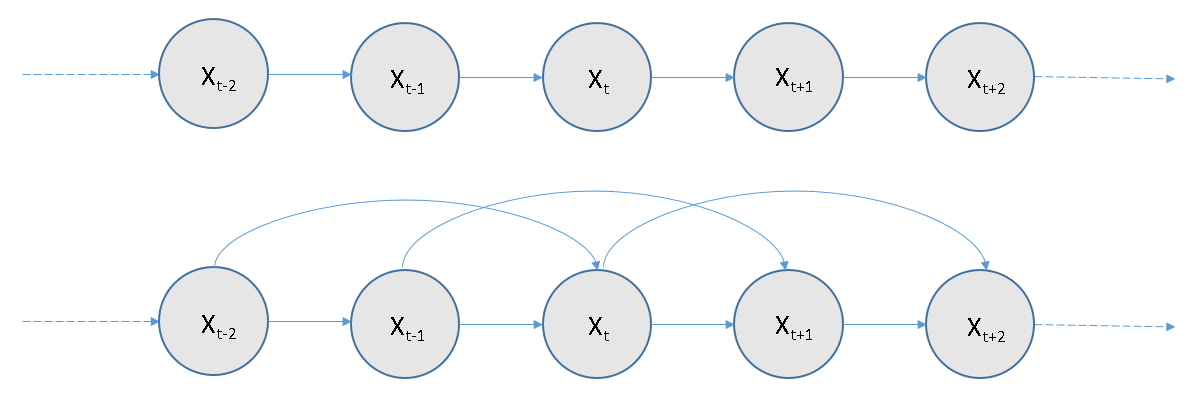
\includegraphics[width=0.8\linewidth]{Chapters/BackgroundKnowledgeAndRelatedWork/MultiAgentTargetDetectionBackground/Figs/MarkovProcesses/MarkovProcesses.png}
    \caption{A graphical model describing first and second order Markov processes}
    \label{fig:markov-processes}
\end{figure}
It also is possible to calculate the probability of the process experiencing a sequence of states from timesteps 1 as far as $t$, using the chain rule of probability and the Markov property:
$P(X_{1:t}) = P(X_1, X_2, ..., X_t) = P(X_1)\times P(X_2 | X_1)\times P(X_3 | X_2, X_1) \times P(X_t | X_{t-1}, X_{t-2}, ... , X_1) = P(X_1) \times \prod_{i=2}^{t}{P(X_i | x_{i-1})}$. Marginalization over variables in this sequence allows the calculation of many useful quantities.
\par

Markov processes can described by graphical models, for example Figure \ref{fig:markov-processes} displays a graphical representation of first and second order Markov processes, where a directed arrow between nodes represents a directional dependence between those nodes.

\subsubsection{HMM Description}\label{subsubsec:HMMDesc}
Hidden Markov Models (HMMs) are models that build on the Markov Process model, which describes the evolution of a random system in the language of probability theory. HMMs assume that the system being modeled can be described by a Markov process, but that the states of this process are unobservable \cite{Ghahramani2001AnNetworks}. This means that it is not possible to determine the state of the system exactly at any given point in time. However, it is possible to make an observation of a random variable that is related to the hidden state which yields information about the hidden state. A graphical representation of a HMM is shown in Figure \ref{fig:hmm}
\begin{figure}[]
    \centering
    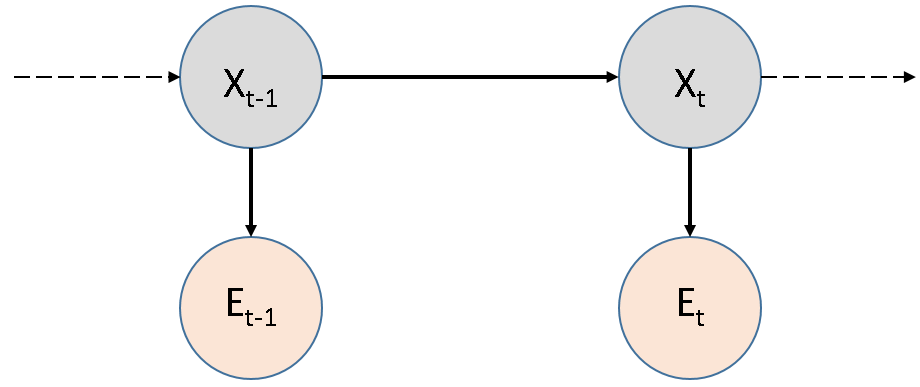
\includegraphics[width=0.8\linewidth]{Chapters/BackgroundKnowledgeAndRelatedWork/MultiAgentTargetDetectionBackground/Figs/HMMs/HMMGraphicalModel.png}
    \caption{A graphical model of a HMM}
    \label{fig:hmm}
\end{figure}
, where the Markov Process is shown by the variables $X_i$ and the observation variables are shown by variables $E_i$. A HMM can be specified by a triple, $\lambda$ = $(T, O, \pi)$, where $T$ is the stochastic transition matrix, $\pi$ is the initial distribution $P(X_1)$ and O describes the conditional probability of an observation given that the system is in a certain state: $O(E_i, X_i) = P(E_{i} | X_{i})$ \cite{Rabiner1989ARecognition}. Taken together, it is then possible to specify the joint distribution of the hidden state variables and the evidence variables, analogous to the Markov Process: 
$
P(X_{1:t}, E_{1:t}) = P(X_1, X_2, ..., X_t, E_1, E_2, ..., E_t) = P(X_1) \times P(E_1 | X_1) \times
\prod_{i=2}^{t}{(P(X_i | x_{i-1}) \times P(E_t | X_t))}.
$Given this representation, it is then possible to answer questions identified in \cite{Rabiner1989ARecognition} and \cite{Murphy1994DynamicLearning}:
\begin{itemize}

    \item Given the HMM, $\lambda$, determine the probability of occurrence of a particular observation sequence, $P(E_{1:t} | \lambda)$
    
    \item Given a sequence of observations $(E_1, E_2, ..., E_n)$, what is the most likely sequence of hidden states that led to these observations? i.e. find \[\argmax_{X_{1:t}} P(X_{1:t} | E_{1:t})\]
    
    \item Determine the parameters of $T$ and $O$, given a training set of observations, i.e. find the solution to \[\argmax_{\lambda} P(E_{1:t} | \lambda)\]
    
    \item \textit{Filtering}: What is the current distribution of the hidden state given all previous evidence ('belief state') of the agent at time t: $P(X_t | E_{1:t})$?
    
    \item \textit{Prediction}: What is the distribution of the hidden state in the future, given all evidence to date: $P(X_{t+k} | E_{1:t})$, for some k$>$0?
    
    \item \textit{Smoothing}: What is the distribution of a past state given all observations up to the current point in time: $P(X_k | E_{1:t})$, for some 0 $\leq$ k $<$ t?
    
\end{itemize}
\par

%Might include a subsection on a taxonomy of commonly used HMMs.

%\subsubsection{Summary}\label{subsubsec:Summary}
%In summary, HMMs can be used to abstractly describe the evolution of a stochastic system. They have been used to achieve state of the art performance in problems such as speech recognition \cite{ChiuSTATE-OF-THE-ARTMODELS} and ... . An comprehensive overview of extensions to the vanilla HMM can be found at \cite{Murphy1994DynamicLearning}.

\subsection{Dynamic Bayesian Networks}\label{subsec:BGDBN}


\begin{wrapfigure}{r}{0.7\textwidth}
    %\centering
    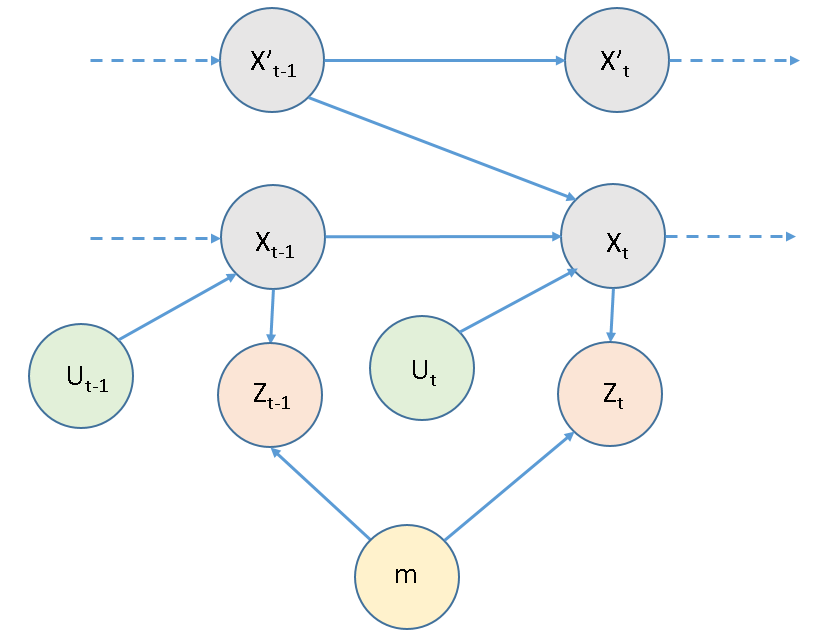
\includegraphics[width = 0.7\textwidth]{Chapters/BackgroundKnowledgeAndRelatedWork/MultiAgentTargetDetectionBackground/Figs/DBNs/Complex2TDBN.PNG}
    \caption{A DBN used for \textbf{S}imultaneous \textbf{L}ocalisation \textbf{a}nd \textbf{M}apping (SLAM), based on \cite[p.~311]{Thrun:2005:ProbabilisticRobotics}.}
    \label{fig:2TDBNExample}
\end{wrapfigure}

DBNs are a generalization of HMMs and are used to model time series. The key difference between DBNs and HMMs is that DBNs are not limited in how they decompose the hidden state variables of a complex stochastic system into the variables that represent its constituent conditional distributions \cite{AIAMA}. Rather than use a single random variable, $X_t$ to represent the state space, a set of random variables are used \cite{Murphy1994DynamicLearning}. DBNs can be considered as a special case of a Bayesian Network with an infinite number of nodes and repeating structure which specifies the transition probabilities between one time step and the next \cite[p.~204]{KollerPGM}. The hidden state variables are represented by nodes which have an associated conditional probability distribution (CPD) which states the probability of observing a value of a random variable given its parents: $p(X_i | Parents(X_i))$, where $i$ is the index of a node in the network \cite[p.~14]{Murphy1994DynamicLearning}. Given this representation, it is possible to calculate the joint distribution, $p(X_t | X_{t-1})$, of all $N$ state variables at time $t$ given the joint distribution at $t-1$ as \cite[p.~14]{Murphy1994DynamicLearning}:
\[
p(X_t | X_{t-1}) = \prod_{i=1}^{N}p(X_t^i | Parents(X_t^i)
\]
$i$ denotes the index of each $N$ variables in the network. \citeauthor{KollerPGM} provide a technical definition of DBNs: 
"\textit{A dynamic Bayesian network (DBN) is a pair $\langle B_0, B_\rightarrow \rangle$, where $B_0$ is a Bayesian network over $X^{(0)}$, representing the initial distribution over states, and $B_\rightarrow$ is a 2-TBN for the process. For any desired time span T $\geq$ 0, the distribution over $X^{(0:T)}$ is defined as a unrolled Bayesian network, where, for any $i$ = 1, . . . , $n$:
\begin{itemize}
    \item The structure and CPDs of $X^{(0)}_i$ are the same as those for $X_i$ in $B_0$,
    \item The structure and CPD of $X^{(t)}_i$ for $t > 0$ are the same as those for $X^{'}_i$ in $B_\rightarrow$.
\end{itemize}}" \cite[p.~204]{KollerPGM}. What this essentially means is that a DBN is a compact way of specifying an infinite set of Bayesian Networks (one for each $T>0$) with repeating structure.


Technically, every DBN can be represented as a HMM and visa versa, however, the number of parameters that need to be determined to represent DBNs can be significantly less than that of HMMs \cite{KollerPGM}. For example, consider the case of $n$ discrete random variables, each with support of size $m$. Specifying the full joint distribution without assuming any conditional independences between variables would require a number of probabilities exponential in the number of random variables, $m^{n}-1$, whereas specifying the same joint distribution as factored conditional distributions may require far fewer, reaching a number of probabilities directly proportional to the number of random variables, $n \times m$ in the degenerate case \cite[p.~63]{KollerPGM}. 
%\subsubsection{A Note on Bayesian Networks}
%A Bayesian Network (BN) is a graphical way to represent a particular factorization of a joint distribution. For a detailed explanation, the reader is referred to \cite{KollerPGM}. To fully explain a complex system, it is often natural to model it as the joint distribution of a number of random variables. This is in general intractable \cite{KollerPGM}. In order to circumvent this, independence properties in the distribution can be exploited to provide a much more compact representation of the distribution. BNs exploit the fact that independence is a strong notion that doesn't often occur in the real-world; however conditional independence is a weaker property that is far more prevalent, which still leads to the desired compact representation. BNs are described by a directed acyclic graph (DAG), $G$. The nodes in the graph correspond to the random variables whose joint distribution is of interest, and the arcs represent conditional independences. Specifically, if one Burglary points to Alarm as in figure \ref{fig:BayesianNetwork}, it is implied that the distribution of Alarm is conditionally independent on all other nodes in the network given Burglary. This means that only local conditional probability distributions must be provided in order to specify the full joint distribution.

%\begin{figure}
%example bayesian network figure
%\begin{tikzpicture}[
%  node distance=1cm and 0cm,
%  mynode/.style={draw,ellipse,text width=2cm,align=center}
%]
%\node[mynode] (i) {Burglary};
%\node[mynode,below right=of i] (g) {Alarm};
%\node[mynode,above right=of g] (c) {Earthquake};
%\path %(ra) edge[latex-] (sp)
%(g) edge[latex-] (c) 
%(g) edge[latex-] (i);
%\node[left=0.45cm of i]
%{
%\begin{tabular}{cM{3}M{3}}
%\toprule
%\multicolumn{2}{c}{Burglary} \\
%\multicolumn{1}{c}{T} & \multicolumn{1}{c}{F} \\
%\cmidrule(r){1-2}
%0.001 & 0.999 \\
%\bottomrule
%\end{tabular}
%};
%\node[right=0.45cm of c]
%{
%\begin{tabular}{cM{3}M{3}}
%\toprule
%\multicolumn{2}{c}{Earthquake} \\
%\multicolumn{1}{c}{T} & \multicolumn{1}{c}{F} \\
%\cmidrule(r){1-2}
%0.008 & 0.992 \\
%\bottomrule
%\end{tabular}
%};
%\node[below=0.5cm of g]
%{
%\begin{tabular}{ccM{2}M{2}}
%\toprule
%& & \multicolumn{2}{c}{Alarm} \\
%\multicolumn{2}{l}{Burglary Earthquake} & %\multicolumn{1}{c}{T} & \multicolumn{1}{c}{F} \\
%\cmidrule(r){1-2}\cmidrule(l){3-4}
%F & F & 0.01 & 0.99 \\
%F & T & 0.95 & 0.05 \\
%T & F & 0.8 & 0.2 \\
%T & T & 0.99 & 0.01 \\
%\bottomrule
%\end{tabular}
%};
%\end{tikzpicture}

%\caption{Simple Bayesian Network based on %\cite[P.~512]{AIAMA}}
%\label{fig:BayesianNetwork}
%\end{figure}



%\subsubsection{Dynamic Bayesian Network Technical Description}



%, which represent a general temporal probability model that describes a random system which is assumed to have a number of random variables, some of which are observable and some not \cite{AIAMA}.
%Dynamic Bayesian networks are usually used to represent the dynamics of a random system over time and can be described generally by specifying how the system transitions from its state at $t-1$ to $t$, if the first order Markov property is assumed. This thesis is concerned with the case when the first order Markov property holds. 
It is often convenient to categorise the random variables in the network into state variables (assumed to be hidden), control variables and observation variables \cite{Thrun:2005:ProbabilisticRobotics}. An example of a Dynamic Bayesian Network can be seen in Figure \ref{fig:2TDBNExample}. The hidden state variables are shaded in light grey, the observation variables in light orange and the control variables in light green. The directed arcs represent "instantaneous" causation, as with regular Bayesian Networks \cite[p.~15]{Murphy1994DynamicLearning}. Note that unlike HMMs, there isn't a requirement to have a single state and observation variable across each time-step and other variables can be introduced into the model.

%The nodes in the graph correspond to the random variables whose joint distribution we would like to calculate, and the arcs represent conditional independences \cite{KollerPGM}. Specifically, if one node points to another. \par













\subsection{Inference Algorithms}\label{subsec:BGInfAlgos}
%\nomenclature[]{MLE}{Maximum Likelihood Estimate}
%\note{Make sure it's clear whether using random variables or not}
%\note{Might need to make clear Markov assumptions }
As discussed, HMMs and DBNs are useful tools for modelling complex random dynamic processes. Typically, models are used to provide some kind of inference about a process, to gain insight into its inner workings. By inference, we mean calculating the probability distributions over variables of interest. Some algorithms will be outlined here that will demonstrate how to calculate both exact and approximate inferences, using general structures for HMMs and DBNs. \par

First, inference algorithms commonly used with HMMs are discussed, as their representation is more rigid, meaning that it is easier to exploit their structure generally to perform inference. As previously stated, HMMs and DBNs are routinely used to model systems that have state variables that cannot be directly observed. In most cases, we are interested in inferring what the state of the system might be, given the observed evidence variables received. This is the first and arguably the most useful inference challenge that we inspect.

The actual quantity that we want to compute is 
\[P(X_t | e_1, e_2, ..., e_t) = P(X_t | e_{1:t})\]
that is, the probability distribution of the hidden state variable, given all previously observed evidence variables. The notation $e_{1:t}$ denotes the joint distribution of $e_1, e_2, ..., e_t$. We are interested in computing this value, rather than the unconditional state distribution, $P(X_t)$, because we cannot observe the state directly, but we can observe the evidence variables. The conditional distribution $P(X_t | e_{1:t})$ is frequently referred to as the \textit{belief state} and the process of calculation of this distribution is frequently referred to as \textit{state estimation} or \textit{filtering} \cite{AIAMA}, \cite{Thrun:2005:ProbabilisticRobotics}, \cite{KollerPGM}. The \textit{forward algorithm} can be used to calculate the value of $P(X_t | e_{1:t})$ \cite[p.~572]{AIAMA}. It is a recursive algorithm, and takes advantage of the fact that the underlying process is Markovian. The forward algorithm for HMMs is shown in Algorithm \ref{alg:forwardAlgorithmHMMs} and is based on the algorithm outlined in \cite[p.~27]{Thrun:2005:ProbabilisticRobotics}. The derivation is useful to follow as an exercise, so we present it in the subsequent sub-section.
\subsubsection{HMM Filtering Algorithm Derivation} 
\label{section:HMMFiltering}
\note{Might be better to put this in an appendix.}
Two well-known probability identities are used in the derivation: 
\note{Fix the formatting here}
\begin{center}
%- - - - - - - - - - - - - - - - - - - - - - - - - - - - - - - - - - - - - - - - - - - - - - - - - - - - - - - - - - - - - 
\end{center}
%quad adds space
\[(a) \quad p(A | B, C) = \frac{p(B | A, C) p(A | C)}{p(B | C)} \quad \text{and} \quad (b) \quad p(A | B) = \int\limits_{C}P(A | B, C) P(C | B)dC\]

\begin{center}
%- - - - - - - - - - - - - - - - - - - - - - - - - - - - - - - - - - - - - - - - - - - - - - - - - - - - - - - - - - - - - 
\end{center}
The derivation is as follows:
\begin{enumerate}
\item {$ p(X_t | e_{1:t}) = p(X_t | e_{1:t-1}, e_t) $ }

\item{$ \text{applying (a) and letting} \quad \eta = \frac{1}{p(e_t | e_{1:t-1})} \quad = \quad \eta p(e_t | e_{1:t-1}, X_t)p(X_t|e_{1:t-1}) $ }

\item{$ \text{by the Markov property} \quad = \quad \eta p(e_t | X_t)p(X_t|e_{1:t-1})$}

\item{$\text{applying (b)} \quad =  \quad \eta p(e_t | X_t)\int_{X_{t-1}}p(X_t|e_{1:t-1}, X_{t-1}) p(X_{t-1}|e_{1:t-1})dX_{t-1}$}

\item{$ \text{by the Markov property} \quad = \quad \eta p(e_t | x_t)\int_{X_{t-1}}p(X_t|X_{t-1}) p(X_{t-1}|e_{1:t-1})dX_{t-1} $}

\end{enumerate}
Note that $\eta$ is a normalizing constant that ensures that the probability distribution integrates to 1, and that the probabilities that need to be calculated can be done so from the parameters specified in the HMM; namely $p(e_t | X_t)$, specified by the sensor model, and $p(X_t | x_{t-1})$, specified by the transition model.

\begin{algorithm}{}
\caption{Forward Algorithm for HMMs}
\label{alg:forwardAlgorithmHMMs}

\begin{algorithmic}[1]
\renewcommand{\algorithmicrequire}{\textbf{Input:}}
\renewcommand{\algorithmicensure}{\textbf{Output:}}
%Input
\REQUIRE $\newline P(x_{t-1} | e_{1:t-1})=bel(x_{t-1}): \quad \text{The belief distribution as far as the previous time-step}
\newline e_t: \quad \text{The most recent observation}
\newline hmm: \quad \text{A Hidden Markov Model specifying the transition and observation probabilities,} \newline p(X_t | x_{t-1}) \text{ and } p(E_t | x_t)$
%Output
\ENSURE  $\newline P(X_{t} | e_{1:t}) = bel(X_{t})$

\hfill\pagebreak

\FOR{all $x_t$}
\STATE $\overline{bel}(x_t) = \int p(x_t | x_{t-1}) p(x_{t-1} | e_{1:t-1}) d x_{t-1}$
\STATE $bel(x_t) = p(e_t | x_t) \overline{bel}(x_t)$
\ENDFOR
\STATE $ \eta = 1 / \int_{x_t}{bel(x_t)}dx_t$
 \FOR{all $x_t$ do:}
\STATE $bel(x_t) = \eta{bel}(x_t)$
\ENDFOR  
    
%\ENDWHILE
\RETURN $bel(X_t)$
\end{algorithmic} 
\end{algorithm}

\note{Don't forget to mention: Sufficient statistics, forward algorithm}

Algorithm \ref{alg:forwardAlgorithmHMMs} uses integrals to account for the fact that the distribution of the hidden state, $X_t$, may be continuous. The work done in this thesis only uses discrete distributions, and so summations are used instead of integrals for the subsequent discussion. A consequence of using discrete distributions is that it is possible to formulate the forward algorithm using vector and matrix notation. As outlined in Section \ref{subsec:BGHMM}, the transition model $T=p(X_t | X_{t-1})$ for a HMM can be written down in matrix form, as can the observation model $O_t=p(E_t | X_T)$. This allows for a highly compact notation: denoting $p(x_t | e_{1:t})$ as $f_{1:t}$, we can write $f_{1:t} = \eta O_{t} T^{T} f_{1:t-1}$, where $f_{1:t}$ contains the vector of values of $p(x_t | e_{1:t})$ for every possible $x_t$ \cite[p.~579]{AIAMA}. Note that the observation model, $O_t$ is time dependent, as opposed to the transition model, which is assumed to be stationary. \par

Some insight can be gained from studying Algorithm \ref{alg:forwardAlgorithmHMMs}. There are three main steps to this algorithm, and the intuition behind them is explained based on explanations in \cite{AIAMA}, \cite{Thrun:2005:ProbabilisticRobotics} and \cite{Murphy1994DynamicLearning}: 
\note{These are highly verbose, edit to make less wordy}
\begin{enumerate}
    
    \item The first step is often referred to as the prediction step:
    \begin{center}
    $\overline{bel}(x_t) = \sum_{x_{t-1}} p(x_t | x_{t-1}) p(x_{t-1} | e_{1:t-1}) d x_{t-1}$
    \end{center}

    This step carries out the first part of the calculation of the belief value for a given state $x_t$, by marginalizing over all possible hidden states ($x_{t-1}$) that could have preceded the current one ($x_t$). This reflects intuition: the probability of being in state $x_t$ should depend on the probability of transitioning from all possible previous states to $x_t$. 
    %\note{this sentence doesn't seem necessary}
    Think "\textit{the probability that I am in location x is the sum of probabilities of starting at all other possible locations and subsequently ending up in location x, weighted against my belief that I began in each other possible location}".
    
    %product of our most recent belief of being in state $x_{t-1}$, given by $p(x_{t-1} | e_{1:t-1})$ and the probability of transitioning from that state to state $x_{t}$, for all previous possible states that we could have been in. 
    $\overline{bel}(x_t)$ effectively projects our current belief to the next time step by using the transition probabilities specified in the HMM.
    
    \item The second step is often referred to as the correction step, or the measurement update step: 
    \begin{center}
    $bel(x_t) = p(e_t | x_t) \overline{bel}(x_t)$ 
    \end{center}
    This step takes the projected belief in step 1 and multiplies it by the probability of observing the data that we did in the given hidden state, $x_t$. This can be thought of as a correction because the use of the measurement data narrows the probabilities of the possible states that the system could have transitioned to. 
    \note{Need to re-word this to make more concise}
    %For example, if the value of a transition probability from state x to state y is low, and there is a low probability that the system was previously in state x, a high probability of observing the observed sensor reading given state y can still result in a relatively high posterior probability of the system being in state y given the new evidence.
    
    \item The final step is to ensure that the distribution sums to 1. This is done by multiplying by a normalizing constant, $\eta$.
    
    
\end{enumerate}
A key strength of this algorithm is the fact it allows updates to be performed online. The reason for this is that the information-state vector, $p(x_t | e_{1:t})$ is a sufficient statistic for the past history of observations. For a full proof of this property, the reader is referred to Appendix A of \cite{Smallwood1973TheHorizon}, which also provides insight into the update rule itself. In relation to the update rule, note that an initial distribution of the estimated state must be provided to this algorithm before the first update can be performed. The complexity of the forward algorithm is $\theta (nm^2)$, where m is the size of the joint distribution of the hidden variables, x, and n is the number of time-steps that have occurred. This is clear to see when viewing the update as the matrix-vector multiplication $f_{1:t} = \eta O_{t} T^{T} f_{1:t-1}$, as the size of T is $m^2$.






\subsubsection{Evidence Likelihood Algorithm Using a HMM}\label{subsubsec:EvLikelihood}
\note{Will talk about this briefly for SPRT}
The second useful quantity that we would like to calculate is the probability of observing the evidence that we did, often referred to the likelihood function of the data, as identified in Section \ref{subsec:BGHMM}. In simpler terms, this is the calculation of the probability of observing the data, given a fixed parameterised model of the data (the HMM). This value is useful as it can reveal insights into whether one model is more likely than another model, with applications including \textbf{M}aximum \textbf{a} \textbf{P}osteriori (MAP) parameter estimates and hypothesis testing. It is used in this thesis in Section \ref{subsubsec:SeachTerminationMethodology}. We would like to compute the value of
\[P(e_1, e_2, ..., e_t) = P(e_{1:t})\]
given the fixed set of parameters provided by the HMM. A brief outline of the derivation is shown:\note{might be best to put the derivation in an appendix} 


\subsubsection{HMM Evidence Likelihood Algorithm Derivation}\label{subsubsec:BGEvidenceLikelihood}

Analogous to the filtering algorithm derivation, two well-known probability identities are used in the derivation: 
\begin{center}
%- - - - - - - - - - - - - - - - - - - - - - - - - - - - - - - - - - - - - - - - - - - - - - - - - - - - - - - - - - - - - 
\end{center}
%quad adds space
\[(a) \quad p(A, B, C) = p(A | B, C) p(B, C) \quad \text{and} \quad (b) \quad p(A, B) = \sum_{C}{p(A | B, C)p(B, C)}\]

\begin{center}
%- - - - - - - - - - - - - - - - - - - - - - - - - - - - - - - - - - - - - - - - - - - - - - - - - - - - - - - - - - - - - 
\end{center}

The derivation is as follows:
\begin{enumerate}

\item {$p(e_{1:t}) = \sum_{x_t}p(e_{1:t}, x_t) \quad = \quad \sum_{x_t}p({e_{1:t-1}, e_t, x_t}) $
}
\item {$\text{applying (a) } \quad= \quad
\sum_{x_t}{p(e_t | e_{1:t-1}, x_t)p(x_t, e_{1:t-1})}$
}
\item{$\text{by the Markov property} 
\quad = \quad \sum_{x_t}p(e_t | x_t)p(x_t, e_{1:t-1})$
}

\item{$\text{applying (b)} \quad =  \quad
\sum_{x_t}p(e_t | x_t) \sum_{x_{t-1}}p(x_t|e_{1:t-1}, x_{t-1}) p(x_{t-1},e_{1:t-1})$
}

\item{$\text{by the Markov property} \quad = \quad 
\sum_{x_t}{p(e_t | x_t)\sum_{x_{t-1}}p(x_t|x_{t-1}) p(x_{t-1},e_{1:t-1})}$
}

\end{enumerate}

The algorithm for calculating likelihoods uses the forward algorithm, $\alpha$, with the replacement of  $p(x_{t-1}|e_{1:t-1})$ with $p(x_{t-1}, e_{1:t-1})$ and one final summation. This means that it is possible to use the forward algorithm to calculate likelihoods: $p(e_{1:t}) = \sum_{i=1}^{n} \alpha(x_i, e_i)$, where $\alpha(x, e)$ is the result of applying the forward algorithm to the sequence of evidence variables $(e_1, ..., e_t)$.


%No point in writing up likelihood algorithm as it's very similar to forward algorithm.

%\subsubsection{HMM Parameter Learning Using Expectation Maximization}\label{subsubsec:EMAlgo}
%\note{Can talk about this briefly for battery model}
%Since a HMM is a parameterised model of a stochastic process, a natural question to ask is whether it is possible to determine a \textit{"best"} set of parameters to describe the process, by using observations of the process. This is a more complex version of the well-known process of finding the parameters that maximize the likelihood function of fully observable data, known as the \textbf{M}aximum \textbf{L}ikelihood \textbf{E}stimate (MLE). Finding the most likely set of parameters which provided the observed values can be described mathematically as the value of \note{fix argmax notation}$\argmax_{\lambda} P(E_{1:t} | \lambda)$. Note that this is a fundamentally different problem to that discussed in the preceding section; here we do not assume a fixed set of parameters for the HMM ($\lambda$).

%This is a well-studied problem for HMMs and the solution is given by the \textbf{E}xpectation \textbf{M}aximisation (EM) algorithm, proposed by \citeauthor{Dempster1977MaximumAlgorithm}. This algorithm is reasonably complex and highly detailed overviews can be found in many texts that deal with parameter estimation for statistical models. A quick outline of how the algorithm works is provided here.\par


%The reason why the standard methods for finding the MLE for a parameterised model do not work with HMMs is due to the fact that there is no way to directly express the quantity  $P(E_{1:t} | \lambda)$ directly. This can be seen in the derivation of the evidence likelihood in <reference whichever appendix it ends up in>. Instead, it is necessary to marginalize over states: $ P(e_{1:t} | \lambda) = \sum_{x_t}{p(x_t, e_{e:t} | \lambda)}$. The standard approach to finding the parameters that maximize a model is to take a log transform of the likelihood function, which preserves the solution but turns the problem into one of finding the parameters that maximize a sum rather than a product. Using standard methods of calculus, this can usually be done easily. The issue with HMMs is that when a logarithmic transformation is applied to the likelihood function, the summation sign remains within the log function, which means finding the maximum is still a difficult problem. The EM algorithm, taking the approach of many iterative techniques, relaxes the constraints on the problem in order to find a lower bound of the log-likelihood and then iteratively improves this lower bound with increasing likelihood values. 


%The Baum-Welch algorithm is a special case of the EM algorithm and is frequently used to solve the problem of estimating the parameters of a HMM. The algorithm is described fully in appendix <reference appendix>.


\subsubsection{Filtering Algorithm for DBNs}\label{subsubsec:filteringDBN}
\note{Extend HMM to add control variable}
\begin{wrapfigure}{r}{0.68\textwidth}
    \centering
    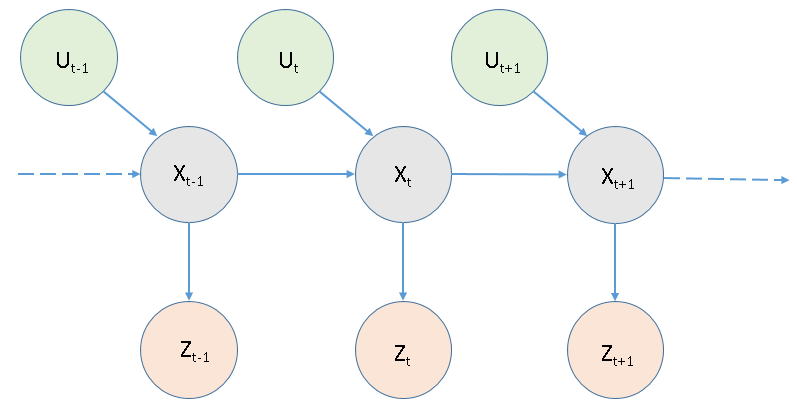
\includegraphics[width = 0.68\textwidth]{Chapters/BackgroundKnowledgeAndRelatedWork/MultiAgentTargetDetectionBackground/Figs/HMMs/HMMWithControl.png}
    \caption{A DBN with Hidden State variables (grey), Observation variables (orange) and Control variables (green).}
    \label{fig:HMMWithControlVariablesExample}
\end{wrapfigure}
The forward algorithm for state estimation was presented in Section \ref{section:HMMFiltering}. A slightly modified version of this algorithm is now described, which is very commonly used in stochastic systems that can be influenced by actions that an agent may take. Such systems have \textit{control variables} as well as hidden state variables and observation variables. These control variables (variables which represent the actions that an agent may perform) have an influence on the transition probabilities between states. The graphical model in Figure \ref{fig:HMMWithControlVariablesExample} describes the basic case. The arrows describe the conditional independence assumptions: at time t, the hidden state ($x_t$) depends on the previous state ($x_{t-1}$), and the previous control action taken ($u_t$). As with the HMM, the observation $e_t$ is conditionally dependent on the state $x_t$. This causes a slight change in the filtering algorithm: on line 2 of algorithm \ref{alg:forwardAlgorithmHMMs}: $\overline{bel}(x_t) = \sum_{x_{t-1}} p(x_t | x_{t-1}) p(x_{t-1} | e_{1:t-1}) $ is replaced with $\overline{bel}(x_t) = \sum_{x_{t-1}} p(x_t | u_t, x_{t-1}) p(x_{t-1} | e_{1:t-1}, u_{1:t-1})$, reflecting that transition probabilities now depend on the most recent control action taken, as well as the previous state.


%DBNs have already been shown to be a powerful tool while modelling stochastic systems, since the hidden variables can be described by conditional independences, rather than 



%This algorithm can be further generalized - if multiple control variables, hidden state variables and observation variables are needed to describe the system fully, it is possible to make minor modifications which reflect the conditional independences stated by the underlying DBN by .

It is worth noting that there are many filtering algorithms that deal with data that come from certain distributions and satisfy constraints related to their transition and observation models, for example the Kalman Filter \cite[p.~43]{Thrun:2005:ProbabilisticRobotics}.






%\subsubsection{Discrete Bayes Filter}
%\note{This is what is used in the work that I did, so it is outlined}

\subsubsection{Approximate State Estimation}
\note{Thought about using Particle filter to avoid the dimensionality problem when attempting to maintain estimated state}
The state estimation algorithms mentioned so far maintain the exact values of the distribution $p(x_t | e_{1:t}, u_{1:t})$, but we will quickly mention an approximate method that is also frequently used. The computational complexity of the filtering algorithms is determined by how well the joint distribution of hidden state variables, observation variables and control action variables can be factored, but in the worst case the complexity is given by the case where the joint distribution of the hidden state variables cannot be factored at all. The forward algorithm, described in Algorithm \ref{alg:forwardAlgorithmHMMs} for a HMM performs the update from each time state in O($n^2$), where $n$ is the dimension of the hidden state variable \cite{Smyth1997ProbabilisticModels}.
%$O(n^2ut)$, where n are the number of hidden states, u is the number of available control actions and t is the number of time steps.
In some cases, this can become intractable if the state space is large enough. % and the transition model cannot be factored. 
In this case, approximate techniques are used. An example is the \textit{particle filter}. Details of the particle filter can be found in \cite[p.~96]{Thrun:2005:ProbabilisticRobotics} and \cite[p.~665]{KollerPGM}.


\subsection{Prediction Algorithms}
\placeholder{}
This contains the details of prediction algorithms

\subsection{Sequential Statistical Hypothesis Testing}\label{subsec:SPRT}
%outlines the background behind the sequential probability ratio test.

\note{This section assumes that the reader has a basic familiarity with the terminology and techniques of hypothesis testing in statistics.}

A statistical test is a mechanism for making quantitative decisions about a process, by determining how well the data stand in agreement with given predicted probabilities \cite{cowan1998statistical}. Statistical tests are usually used to draw conclusions about a \textit{statistical hypothesis}, which is a testable hypothesis based on observations of a process that is modelled using random variables. There are many texts that outline the statistical tests that can be used to make a decision between accepting and rejecting the null hypothesis, $H_0$, for example \cite{IntroductionToMathematicalStatistics}. The usual context in which this occurs is one in which the data has been collected in advance and the sample size is fixed and known. The standard procedure for testing a simple hypothesis involves using a Uniformly Most Powerful (UMP) Test for a fixed value of the probability of making a Type \Romannum{1} error, $\alpha$ \cite[p.~253]{IntroductionToMathematicalStatistics}. The subsequent sections discuss how this can be extended to a sequential paradigm, where the sample size is not fixed.\note{An example might be of value here} \par

There exists a branch of statistical hypothesis testing called \textit{sequential hypothesis testing}, which is used when the sample size is not fixed in advance \cite[p.~375]{IntroductionToMathematicalStatistics}. Given a hypothesis to test, $H_0$, this means the decision process goes beyond deciding whether to accept or reject the null hypothesis, but to either
\begin{enumerate}
    \item Accept the hypothesis being tested, $H_0$.
    \item Reject the hypothesis being tested, $H_0$
    \item Continue the experiment by making a further observation.
\end{enumerate}

It is clear that samples are gathered as long as 1). or 2). above are not chosen, which intuitively corresponds to the notion of making an informed decision, where it is desirable to ensure that enough data has been gathered to draw a meaningful conclusion. In the sequential testing paradigm, two kinds of error may be committed, as with the non-sequential case: we may reject the null hypothesis when it is true (commit a Type \Romannum{1} error) or we may accept the null hypothesis when some alternative hypothesis is true (commit a Type \Romannum{2} error). 

The Sequential Probability Ratio Test (SPRT), which was devised by \citeauthor{Wald1945SequentialHypotheses}, proposes a statistical test for simple hypotheses with specified fixed values, which ensures that the probability of Type \Romannum{1} and Type \Romannum{2} errors do not exceed $\alpha$ and $\beta$ respectively \cite{Wald1945SequentialHypotheses}. \citeauthor{Wald1948OptimumTest} proved that the SPRT is optimal, in the sense that of all tests with the same power, the SPRT requires on average the fewest number of observations to reach a decision \cite{Wald1948OptimumTest}. A strong advantage of the test is that it can be carried out without determining any probability distributions whatsoever \cite{Wald1945SequentialHypotheses}. The SPRT can be thought of as a stopping rule for sampling in a stochastic process. For the sake of brevity, we omit the full derivation of the rule and the proof of optimality, but instead refer the reader to \cite{Wald1945SequentialHypotheses}, \cite{Wald1950BayesProblems} and \cite{Wald1948OptimumTest}. The SPRT can be carried out following the procedure shown in Algorithm \ref{alg:SPRT}.


%\begin{enumerate}
%    \item The null and alternative hypotheses are stated, $H_0$ and $H_1$.
%    \item The desired type \Romannum{1} and type \Romannum{2} error rates are specified as $\alpha$ and $\beta$.
%    \item Calculate the values $A = \frac{1-\beta}{\alpha}$ and $B = \frac{\beta}{1-\alpha}$
%    \item 
%\end{enumerate}


\begin{algorithm}{}
\caption{The Sequential Probability Ratio Test Algorithm}
\label{alg:SPRT}

\begin{algorithmic}[1]
\renewcommand{\algorithmicrequire}{\textbf{Input:}}
\renewcommand{\algorithmicensure}{\textbf{Output:}}
%Input
\REQUIRE $\newline \alpha \text{: \quad The upper limit in probability for making a type \Romannum{1} error.}$
\newline $\beta \text{: \quad The upper limit in probability for making a type \Romannum{2} error.}$
\newline $H_0 \text{: \quad The null hypothesis.}$
\newline $H_1 \text{: \quad The alternative hypothesis.}$
\newline $(x_1, ..., x_m) \text{: \quad The m observations made so far.}$
%Output
\ENSURE  $\newline$ A decision to accept $H_0$, accept $H_1$ or make another observation.\\
\hfill\pagebreak

\STATE Calculate $p_{0m}=p_{0m}(x_1, ..., x_m)$, the probability of observing the data under the assumption $H_0$ is true.

\STATE Calculate $p_{1m}=p_{1m}(x_1, ..., x_m)$, the probability of observing the data under the assumption $H_1$ is true.

\STATE Calculate the values $A = \frac{1-\beta}{\alpha}$ and $B = \frac{\beta}{1-\alpha}$

\STATE Accept $H_1$ if $\frac{p_{1m}}{p_0m} \geq A$

\STATE Accept $H_0$ if $\frac{p_{1m}}{p_0m} \leq B$

\STATE Make an additional observation if $B < \frac{p_{1m}}{p_0m} < A$



\end{algorithmic}
\end{algorithm}


The main idea, as is the case with simple non-sequential hypothesis tests, is based on the idea that if the likelihood ratio ($\frac{p_{1m}}{p_{0m}}$) lies in some \textit{critical region}, $C$, then we may reject the null hypothesis \cite{IntroductionToMathematicalStatistics}. The SPRT extends this by partitioning the m-dimensional sample space $M_m$ into three mutually exclusive regions, $R_m^0$, $R_m^1$ and $R_m$. After the $i_{th}$ observation $(x_i)$ has been drawn, $H_0$ is accepted if $(x_1, ..., x_i)$ lies in $R_m^0$, $H_1$ will be accepted if $(x_1, ..., x_i)$ lies in $R_m^1$ or a $i+1_{th}$ observation will be drawn if $(x_1, ..., x_i)$ lies in $R_m$ \cite{Wald1945SequentialHypotheses}. The process of how to choose $R_m^0$, $R_m^1$ and $R_m$ is outlined in Section 3 of \cite{Wald1945SequentialHypotheses}, which goes beyond the scope of this thesis. The derivation essentially shows that $(x_1, ..., x_i) \in R_m^0$ is equivalent to $\frac{p_{1m}}{p_0m} \leq B$, $(x_1, ..., x_i) \in R_m^1$ is equivalent to $\frac{p_{1m}}{p_0m} \geq A$, and $(x_1, ..., x_i) \in R_m$ is equivalent to $B < \frac{p_{1m}}{p_0m} < A$.

\subsubsection{Summary}
The SPRT is a sequential hypothesis test that formulates a stopping rule in order to draw conclusions based on statistical data. It has frequently been in quality control studies, where samples can be expensive to gather, but it can be applied in other scenarios where sampling can be expensive \cite{Ou2010AnMean}. We use it in Section \ref{subsubsec:SeachTerminationMethodology}

\subsection{Related Literature}
\workinprogress

A problem explored in this thesis is an instance of target detection using a system of aerial robots. A more primitive version of this problem initially gained traction in the literature with the work of Koopman \cite{KoopmanTheoryOfSearchTargetDetection} and has received much attention since. More recent papers have framed the problem in terms of agents and multi-agent system. %Citations needed
A common feature in the problem definition in the literature is that the system of agents are assumed to work in a partially observable environment\cite{Symington2010ProbabilisticUAVs}, \cite{Chung2008Multi-agentFramework}, \cite{WongMulti-vehicleTargets}. Many recent approaches follow the groundwork laid by Elfes\cite{ElfesUsingNavigation}, whereby an "occupancy field" is used to represent the distribution of the target over the cells of a spatial lattice. Elfes describes an Occupancy grid as a "probabilistic tesselated representation of spatial information". This is in contrast to previous approaches that typically used geometric models of the world, which enforced strong domain-specific dependencies. The occupancy field framework 
\par

\section{Multi-Agent Coverage Problem}
\input{Chapters/BackgroundKnowledgeAndRelatedWork/MultiAgentCoverageBackground/MultiAgentCoverageReview.tex}



